\documentclass{article}
\usepackage{geometry}
\usepackage{hyperref}
\usepackage{fancyhdr}  
\usepackage{graphicx}
\usepackage{amssymb}
\usepackage{algorithmic}
\usepackage{algorithm}


\geometry{
  top=1in,
  bottom=1.5in,
  left=1.25in,
  right=1.25in
}

\title{Rapport de projet IA41 - Rasende Roboter}
\author{SENGEL Noé, POURCINE Mattéo, FLEURET Gabriel}
\date{\today}


\begin{document}

\maketitle

\tableofcontents
\newpage

\section{Mise en contexte}
Le but de ce projet est de mettre en application les différents algorithmes vus en cours pendant le semestre d'automne 2023 en \textbf{IA41} (\href{https://fr.wikipedia.org/wiki/Algorithme_de_parcours_en_largeur}{Breadth-First Search}, \href
{	https://en.wikipedia.org/wiki/A*_search_algorithm}{A*}, \href{https://en.wikipedia.org/wiki/Depth-first_search}{Depth-first search}).\\
Ces algorithmes vont être appliqués sur un jeu de société allemand, \href{https://fr.wikipedia.org/wiki/Ricochet_Robots}{\textbf{Rasende Roboter}} ou \href{https://fr.wikipedia.org/wiki/Ricochet_Robots}{Ricochet Robots} en français, créé en 1999 par \href{https://fr.wikipedia.org/wiki/Alex_Randolph}{Alex Randolph}.\\
\\
Nous étions trois à réaliser ce projet. Pour nous permettre de s'organiser au mieux, nous avons choisi de faire un répertoire \href{https://github.com/Glenrunc/IA41_Rasende_Roboter}{\textbf {Github}}. Notre raisonnement a été assez simple concernant l'approche du projet. Nous avons décidé d'implémenter premièrement le jeu pour ensuite y incorporer les algorithmes de résolution.\\\\
Pour la suite du rapport, "Intelligence artificielle" sera remplacée par "IA".
\section{Implémentation du jeu}
Nous avons fait le choix de prendre la première version du jeu. En effet une autre est apparu en 2003, qui ajoutait un robot noir, une case mission multicolore et des agencements de murs différents.
\subsection{Règles du jeu}
Les règles sont assez simple. Le joueur dispose d'un plateau de 16x16 cases. Sur celui-ci est disposé 4 robots de couleurs différentes (rouge, vert, bleu et jaune) et des jetons "missions". Une case centrale permet d'afficher la mission à atteindre par le robot de la couleur de celle-ci.\\ Le but est pour le joueur d'atteindre la mission avec le robot de la couleur correspondante en un minimum de coup et un minimum de temps. Pour cela il peut déplacer tous les robots comme il le souhaite.\\\\
\begin{figure}[h]
  \centering  
  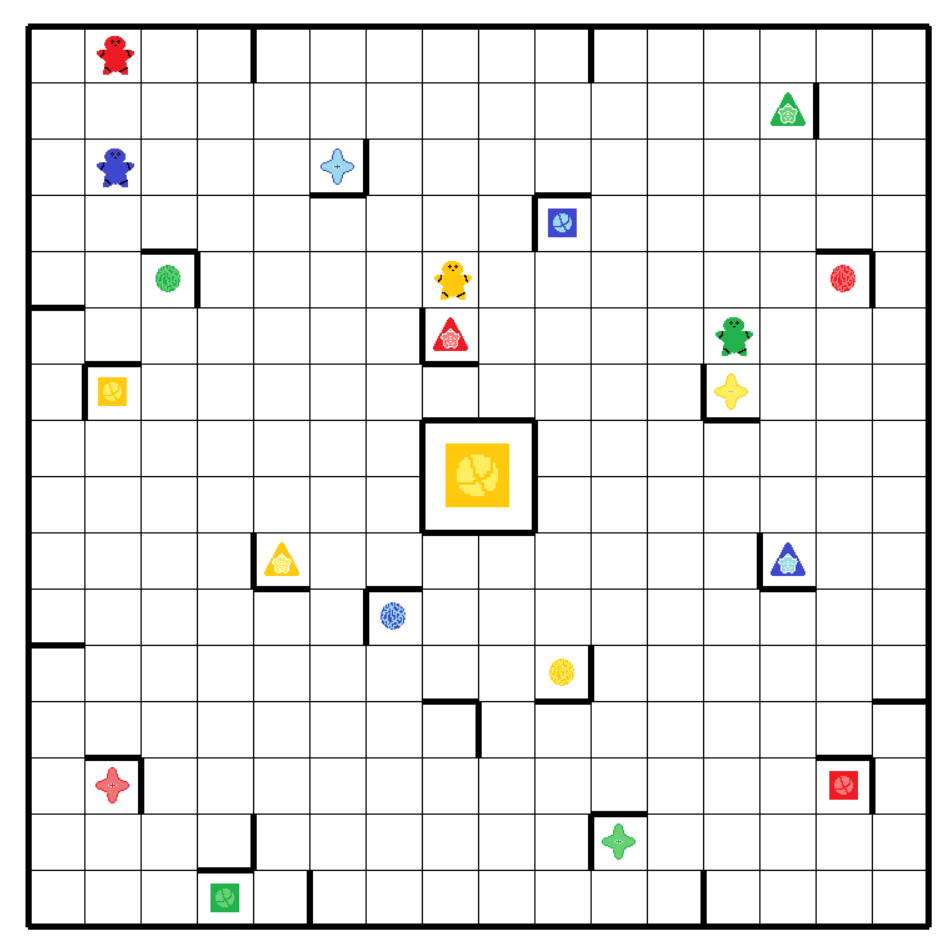
\includegraphics[width=0.5\textwidth]{map_rasende.png}  
  \caption{Image du plateau de jeu "Rasende Roboter"} 
  \label{fig:Plateau}  
\end{figure}
\\
Les déplacements sont assez simple également. Les robots ne peuvent suivre que 4 directions (haut, bas, gauche, droite). De plus une fois qu'une direction est prise, le robot en question ne s'arrête que lorsqu'il croise un mur ou un autre robot.\\\\Chaque partie commence par le tirage d'une mission. Une fois la mission choisit, un compte à rebours est lancé. Pendant ce temps les différents joueurs analysent la position de chaque robot et essayent, dans leur tête, de trouver un moyen de résoudre le problème. Pour faciliter la compréhension, si on regarde la Figure 1, le robot jaune doit atteindre la cible affichée au centre du plateau. Ici elle se situe aux coordonnées (7,2).\\\\
Si un joueur à une solution, il fait signe et donne sa réponse. Si elle est bonne, il gagne, sinon les autres tentent de résoudre le problème.
\subsection{Choix et explications de notre implémentation}
Le but du projet étant d'implémenter différents algorithmes de résolutions, il nous est paru évident de modifier certains points du jeu.\\\\Dans la version physique, le jeu se joue à plusieurs, chacun pour soi. Nous avons décidé que notre jeu pouvait se jouer seul ou à plusieurs contre les algorithmes de résolutions. Ainsi le but de chaque partie est de résoudre le problème en moins de coups possibles certes, mais surtout en moins de coups que ces algorithmes.\\\\Lorsqu'on arrive sur le jeu, on peut choisir la difficulté de l'IA (easy, medium, hardcore).\\\\On peut également choisir de "reset" la manche si on voit que l'on bloque. Un mode revisionnage a été implémenté pour voir les coups effectués par l'IA. Ce mode est uniquement disponible lorsque la manche est terminée et que l'IA a trouvé une solution.\\\\
Au niveau de l'ergonomie de jeu. Il se joue uniquement grâce à une souris ou un pavé tactile. Lorsque l'on clique sur un robot, un chemin s'affiche pour aider le joueur à voir les cases atteignables. Ensuite il peut cliquer sur les différents chemins possibles pour déplacer le robot. 
\begin{figure}[h]
  \centering  
  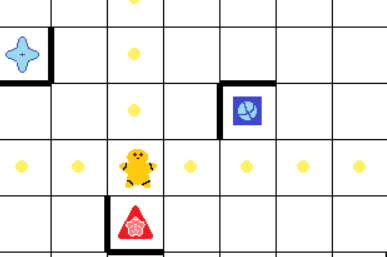
\includegraphics[width=0.5\textwidth]{deplacement.png}  
  \caption{Exemple de déplacement du robot jaune} 
  \label{fig:Plateau}  
\end{figure}\\
Pour ce qui est de l'implémentation du jeu uniquement, nous vous détaillerons certaines méthodes dans la partie réservée aux algorithmes de résolution. Mais pour le reste, nous avons décidé de faire uniquement un diagramme de classes pour rendre plus visuel nos explications.
\begin{figure}
  \centering  
  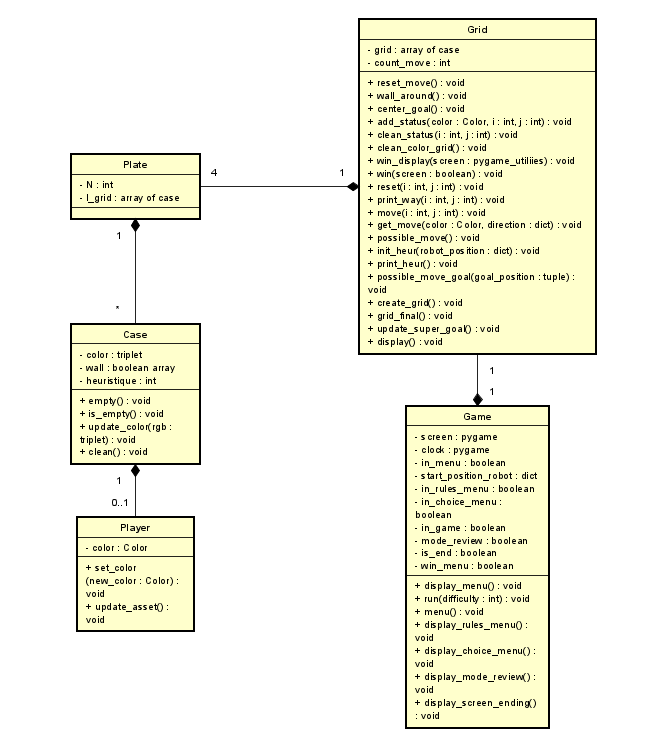
\includegraphics[width=1\textwidth]{diagram_class.png}  
  \caption{Diagramme de classes du jeu Rasende Roboter} 
  \label{fig:Diagram}  
\end{figure}\\
\section{Algorithmes de résolution}
Le jeu, Rasende Roboter, est à la fois un problème de \textbf{planification} et à la fois un problème de \textbf{décision séquentielle}. Plus précisément un problème de planification résolu de manière séquentielle.\\\\
Avant de commencer à implémenter la résolution, il nous a fallu \textbf{comprendre} le problème. Cette étape à été plutôt simple grâce aux règles du jeu. Les \textbf{données} du problème sont : 
\begin{enumerate}
\item  la position des murs dans la grille
\item  la couleur, l'identité et les coordonnées de la mission à atteindre dans la grille
\item  la couleur et les coordonnées des robots 
\item  les déplacements possibles des robots
\end{enumerate}
\textit{Notons que (1) et (4) peuvent être fusionnés en une unique donnée.}\\\\
Ensuite la \textbf{condition} de résolution du problème est la suivante : le robot de la couleur de la mission à atteindre doit se situer sur les coordonnées de cette mission. Ce problème ne présentait pas d'\textbf{inconnues} mise à part le choix de la mission à atteindre en début de partie.\\\\Une fois toutes ces étapes de reconnaissance effectuées et toutes les zones d'ombres écartées, il nous a fallu \textbf{élaborer un plan de résolution du problème}. Nous avons utilisé une approche \textit{\textbf{"Divide and Conquer"}} pour y voir plus clair et résoudre plus efficacement ce problème.
\subsection{Travail préliminaire}
La première partie de notre travail a été d'implémenter le jeu tout en gardant à l'esprit l'ajout des algorithmes de résolutions. En effet un mauvais démarrage aurait été chronophage par la suite alors que l'inverse nous a permis d'être très efficace.\\\\
En implémentant le jeu, il nous a fallu un moyen d'extraire les \textbf{données} explicitées (\textit{\textbf{voir 3}}) lors de notre préparation. L'élément central de notre implémentation est la classe "grid" (\textit{\textbf{voir Fig:3}}). En effet les méthodes suivantes permettent d'extraire des données cruciales.
\begin{itemize}
\item actualize\_robot\_position() permet de créer un dictionnaire, position\_robot, ayant pour clefs la couleur de chaque robot et pour valeurs leur coordonnée dans la grille. 
\end{itemize}
Ainsi lors de l'appel de cette méthode, le dictionnaire suivant est créé, enregistrant à l'instant t la position de chaque robot. Le point (3) a été résolu.
\begin{figure}[!h]
  \centering  
  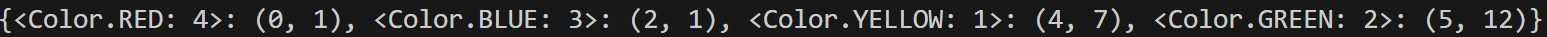
\includegraphics[width=1\textwidth]{dict_pos.png}  
  \caption{Dictionnaire position\_robot} 
  \label{fig:Dict}  
\end{figure}\\\\\\\\\\\\\\\
Ensuite pour résoudre le point (2) nous avons créé un tableau statique de missions sous cette forme.
\begin{figure}[htbp]
  \centering  
  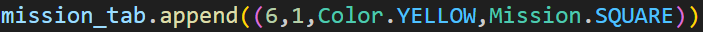
\includegraphics[width=0.5\textwidth]{mission.png}  
  \caption{Tableau de missions} 
  \label{fig:Mission}  
\end{figure}\\
Ainsi lorsque l'on initialise la grille on peut remplacer ses attributs goal\_coordinate et color\_goal par les élements du tableau statique de missions, en tirant aléatoirement une position dans le tableau.\\\\
Les points (1) et (4) ont été les plus délicats. Ils impliquent une multitude de méthodes de la classe "grid".\\\\ Le but était d'avoir une méthode qui initialisait un dictionnaire qui avait pour clefs la couleur de chaque robot et pour valeur une liste de dictionnaires de case atteignable avec pour clefs la direction et pour valeur la coordonnée de la case. Si cela vous paraît trop compliqué voici un exemple.
\begin{figure}[htbp]
  \centering  
  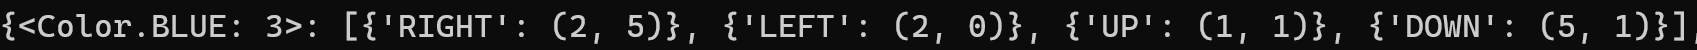
\includegraphics[width=0.9\textwidth]{possible_move.png}  
  \caption{Mouvements possibles par robot} 
  \label{fig:Mission}  
\end{figure}\\
Pour arriver à ce résultat il faut actualiser la position des robots dans la grille grâce à la méthode actualize\_robot\_position() et ensuite il faut voir sur les 4 directions (UP, RIGHT, DOWN, LEFT) quels chemins peuvent emprunter le robot.\\\\ 
Pour cela on se sert de deux informations. La première c'est que le robot avance jusqu'à ce qu'il croise un mur. Pour cette condition il suffit de regarder l'attribut "wall" de la classe "case" qui est un tableau de 4 booléens représentant la présence ou non de mur respectivement dans les 4 directions à une case donnée de la grille.\\\\
Ainsi si le robot veut aller en haut, il suffit de le faire avancer jusqu'à ce que la case sur laquelle il est, contient un mur dans la direction "UP" du tableau de booléen "wall". Il suffit de vérifier  " wall[0] == True ? Stop : Continue ".\\\\
La deuxième information est la suivante. Un robot peut arrêter sa progression si il croise un autre robot sur son chemin.\\\\ Cette condtion est assez simple à verifier si on se sert du dictionnaire position\_robot. On fait avancer le robot dans une direction en vérifiant à la n-ième "case + 1" qu'un autre robot ne s'y trouve pas. Si c'est le cas, on s'arrête, sinon on continue. 
\subsection{Représentation d'un état}
Pour résoudre ce problème, il a fallu définir la représentation \textbf{d'un état} qui permettait d'illustrer l'entièreté de notre problème à un instant donné.\\\\ 
Grâce à notre travail préliminaire, un état à l'instant t sera représenté par le dictionnaire vu à la figure 4. Il ne faut pas oublier que la position des robots ne vaut rien sans la grille correspondante. \\\\
Ensuite il nous a fallu définir \textbf{un système de production}. Pour cela, on se servira du dictionnaire vu à la figure 6.\\\\
Il a fallu ensuite définir un \textbf{état initial} et un ou des \textbf{état/s final/finaux}. Pour cela il suffit de prendre la position de départ de chaque robot (figure 4) pour l'état initial.\\\\
Pour les états finaux il suffit que la robot de la couleur de la mission soit sur les coordonnées de celle-ci et ça peu importe où se trouvent les autres robots.\\\\
Une fois tout ce travail effectué, il faut maintenant appliquer \textbf{des stratégies de résolutions}.
\subsection{Stratégies de recherche dans un arbre}
\subsubsection{Représenter les mouvements du jeu}
Pour résoudre un problème du jeu Rasende Roboter, il faut produire des états à l'instant t + 1 valident à partir d'un état à l'instant t. Ces états produits sont liés à leur état père. Si on applique ce raisonnement sur chaque état produit à l'étape t + 1, t + 2 , etc... On se retrouve à constuire une arborescence de tous les coups possibles pour chaque robot au cours de la partie. La racine de cette arbre sera alors \textbf{l'état initial} et le but sera alors de chercher un des \textbf{états finaux} dans l'arborescence.
\begin{figure}[htbp]
  \centering  
  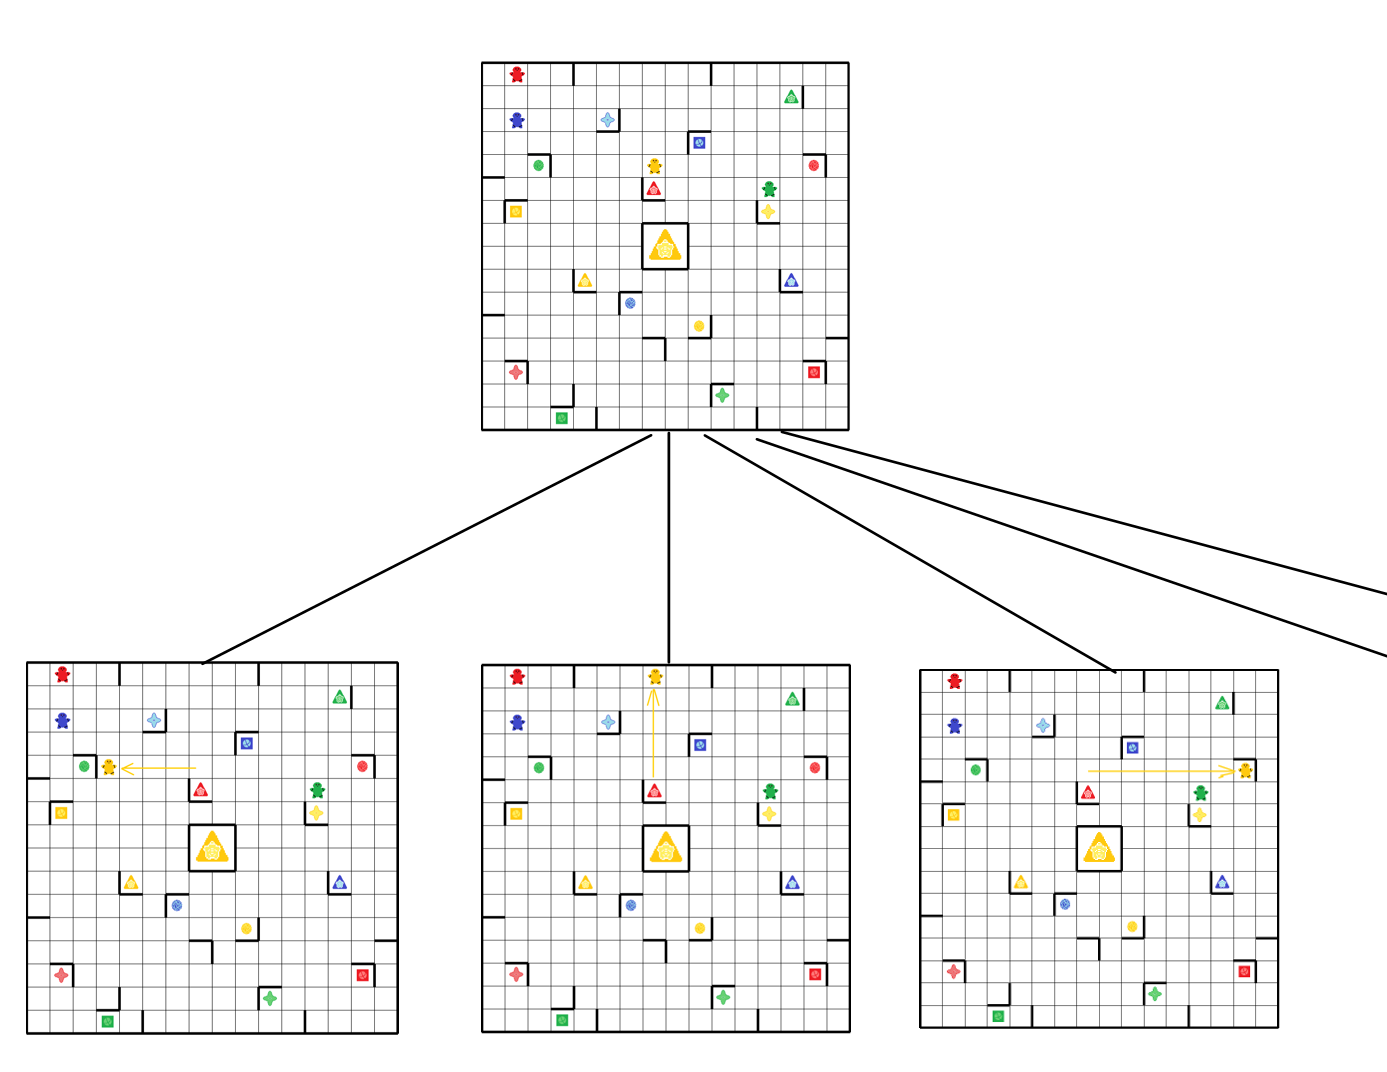
\includegraphics[width=1\textwidth]{arbre.png}  
  \caption{Construction de l'arborescence} 
  \label{fig:Arborescence}  
\end{figure}\\
Chaque étage de l'arbre représente le nombre de déplacements depuis l'état initial. La figure 7 montre l'état au niveau n = 0 et les états au niveau n = 1. Faisons maintenant un peu de mathématiques, si chaque robot peut se déplacer dans les 4 directions à chaque tour. Sachant qu'il y a 4 robots sur le plateau. Les états au niveau n = 1 seront au nombre de 16 car 4 x 4 = 16.\\\\
Maintenant si on suppose qu'au niveau n = 2 chaque état du niveau n = 1 peut encore générer 16 autres états. On aura 16 x 16 = 256 + 1 états dans l'arbre générer. Et cela seulement pour vérifier toutes les configurations possibles en deux coups.\\\\
Bien sûr, chaque état ne génère pas tout le temps 16 autres états car certains robots ne peuvent que faire certains déplacements suivant leur position.\\\\
Mais en extrapolant, on voit vite la croissance exponentielle du nombre d'états générés suivant le nombre de coups nécessaires à la résolution du problème. En règle générale, le nombre d'états selon le nombre de coups n se calcul:\\ \[\forall n \in \mathbb{N^*} , 16^{n} + 1\] \\
\textbf{Comment à partir d'un état, peut-on générer les autres états ?}\\\\
Ceci est plutôt simple, en se servant de la méthode de la classe "grid" possible\_move() , des dictionnaires position\_robot et possible\_move\_per\_robot.\\\\
En effet quand on arrive sur un état on actualise la position des robots pour être à jour, ensuite on parcourt le dictionnaire possible\_move\_per\_robot et on créer un nouvel état en remplaçant uniquement une coordonnée d'un robot et en gardant les autres coordonnées intactes.\\\\
Puis on suit cet algorithme pour générer autant d'états que l'on veut. La fonction next\_state() dans le fichier bfs\_dfs.py est chargée de ce processus de création d'état.\\\\
Deux fonctions pratiques ont été implémentées pour la fonction next\_state(). add\_status\_empty\_grid() et clean\_all\_status() qui permettent respectivement d'ajouter à partir d'un dictionnaire de la forme du dictionnaire position\_robot les robots sur la grille et de retirer les robots de la grille.\\\\
Ainsi pour la suite une seule grille suffira pour tous les traitements et tous les algorithmes de résolutions. Ce qui préserve le stockage en mémoire durant l'éxécution.\\\\
Maintenant que tous les problèmes liés à la représentation des états ont été réglé, nous pouvons passer aux choses sérieuses.
\subsection{Breadth First Search : BFS}
Pour résoudre une partie de Rasende Roboter, il suffit maintenant de constuire l'arbre des états dynamiquement et de le parcourir pour trouver un des états finaux.\\\\
Le breadth first search ou largeur d'abord en français est un algorithme de recherche dans un arbre qui dans notre cas nous permettra de trouver, si solution il existe, le meilleur état final possible. C'est à dire celui en moins de coups. Ci-dessous, l'algorithme du BFS.

\begin{algorithm}
\caption{Breadth First Search}
\label{alg:bfs-reach}
\begin{algorithmic}[1]
  \STATE Entrée: noeud racine $N$
  \STATE Créer FIFO $Q$, Créer Liste $L$
  \STATE $Q$.append$(N)$
  \WHILE{$Q$ n'est pas vide et que le but ne soit pas atteint}
    \STATE Enlever $N$ en tête de liste
    \STATE Ajouter $L$.append$(N)$
    \FOR{tous les fils de $N$, noté $f$}
      \STATE $f$.père = $N$
      \STATE $Q$.append$(f)$
    \ENDFOR
  \ENDWHILE
  \STATE Si le but a été trouvé retourner Succès sinon retourner Echec

\end{algorithmic}
\end{algorithm}
Après avoir implémenté l'algorithme. Nous avons pu effectuer les premiers essais. Pour être rigoureux nous avons mesuré le temps que prenait l'algorithme pour trouver une solution, le nombre d'états parcouru et ainsi le nombre d'états parcouru par seconde.
\\\\
Mais nous avons vite remarqué les limites de cette méthode. Sans améliorations il était presque impossible de trouver des solutions à plus que 7 coups. On le rappel chercher une solution à 7 coups revient au pire des cas à constuire et visiter un arbre de 16 x 16 x 16 x . . . x 16 ( 7-fois ) + 1 états soit 268 435 457 états.\\\\
Au meilleur de sa performance notre algorithme visitait 5000 états / seconde. Pour 7 coups il lui aurait fallu 268 435 457 / 5 000 = 53 687 secondes soit 14 heures pour tenter de trouver cette solution. Ceci n'est pas raisonnable et bien souvent il y avait un stack overflow au bout d'un certain temps d'interprétation.
\subsubsection{Améliorations : BFS}
Nous avons ensuite vu que les solutions qu'il trouvait rapidement étaient celles nécessitant le déplacement d'un seul robot. Nous avons donc réduit la génération des états. La fonction is\_already\_visited() permet de générer seulment les états où un robot n'est pas passé. Ainsi les 4 robots vont aller sur toutes les cases possibles une unique fois. De plus, au lieu de vérifier si le noeud qu'on traite est le noeud final. On vérifie à la génération de chaque état si celui n'est pas un état final. Ainsi on s'évite la vérification et la génération inutile d'états.\\\\
Avec toutes ces améliorations voici un exemple sur un échantillon, même cible mais avec les paramètres différents sur la vérification.
\begin{figure}[!h]
  \centering  
  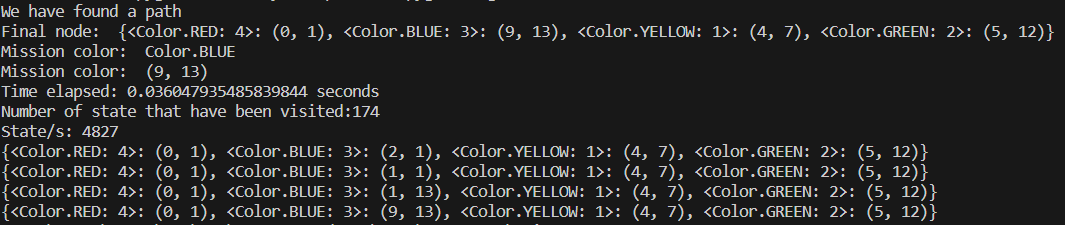
\includegraphics[width=1\textwidth]{sans_verif_generation.png}  
  \caption{BFS sans la vérification à la génération} 
  \label{fig:Diagram}  
\end{figure}\\
\begin{figure}[!h]
  \centering  
  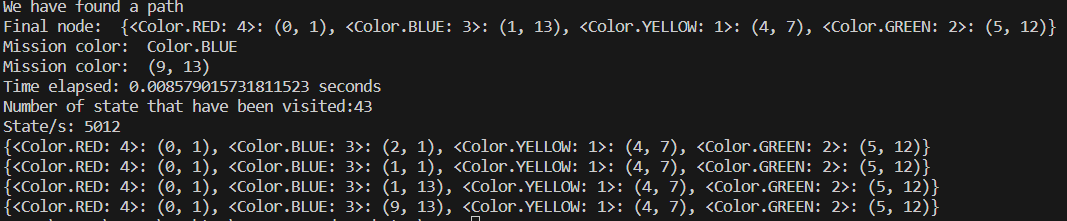
\includegraphics[width=1\textwidth]{avec_verif_generation.png}  
  \caption{BFS avec la vérification à la génération} 
  \label{fig:Diagram}  
\end{figure}\\
On peut voir que la vérification à la génération épargne la visite de 131 états, ce qui permet d'augmenter la vitesse de résolution avec un rapport de 3,75 ce qui n'est pas négligeable.\\\\
Pour conclure notre BFS permet de résoudre 80 \% des problèmes sur la grille fournit dans notre jeu. Le niveau de difficulté associé dans le jeu sera "Medium".
\subsection{Depth First Search : DFS}
En ce qui concerne le depht first search, son implémentation a été rapide puisque son principe est le même que le breadth first search mais au lieu de parcourir l'arbre en largeur , le DFS lui le parcours en profondeur. La solution trouvée sera alors avec un nombre de coups beaucoup plus élevés. Voici son algorithme.
\begin{algorithm}[H]
\caption{Depth First Search}
\label{alg:dfs-reach}
\begin{algorithmic}[2]
  \STATE Entrée: noeud racine $N$
  \STATE Créer LIFO $Q$, Créer Liste $L$
  \STATE $Q$.append$(N)$
  \WHILE{$Q$ n'est pas vide et que le but ne soit pas atteint}
    \STATE Enlever $N$ en tête de liste
    \STATE Ajouter $L$.append$(N)$
    \FOR{tous les fils de $N$, noté $f$}
      \STATE $f$.père = $N$
      \STATE Ajouter en tête de $Q$,les fils notés $f$
    \ENDFOR
  \ENDWHILE
  \STATE Si le but a été trouvé retourner Succès sinon retourner Echec
\end{algorithmic}
\end{algorithm}
\subsubsection{Améliorations : DFS}
Les mêmes améliorations que le BFS ont été implémenté. Il faut néanmoins noter que cet algorithme est plus adapté lorsque l'arbre de recherche a un grand facteur de branchement c'est à dire lorsque le nombre de noeuds au niveau suivant est plus important que celui au niveau actuel. Ce qui est notre cas ici.
\begin{figure}[!h]
  \centering  
  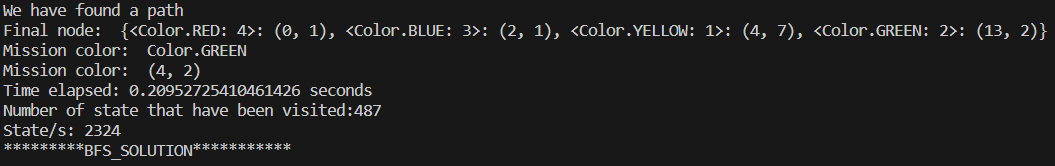
\includegraphics[width=1\textwidth]{bfs_solution_green.png}  
  \caption{Algorithme BFS sur la cible verte en (4,2)} 
  \label{fig:Diagram}  
\end{figure}\\
\begin{figure}[!h]
  \centering  
  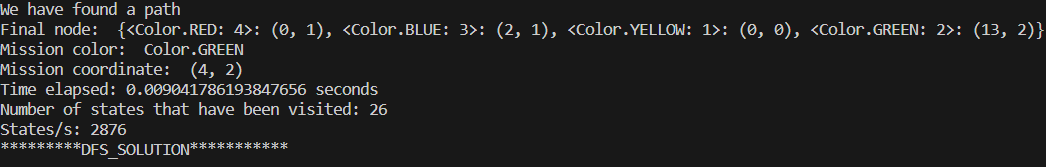
\includegraphics[width=1\textwidth]{dfs_solution_green.png}  
  \caption{Algorithme DFS sur la cible verte en (4,2)} 
  \label{fig:Diagram}  
\end{figure}\\
On le voit mieux sur cet exemple ici, sur une même cible, le DFS parcours seulment 26 états contre 487 pour le BFS pour trouver une solution. Certes, le DFS propose une solution en 26 coups contre 5 pour le BFS. Mais le DFS va environ 23 fois plus vite que le BFS.\\\\
Le DFS sera le niveau de difficulté "Easy" dans notre jeu puisque qu'il propose des solutions avec un grand nombre de coups.
\subsection{A*}
L'objectif de l'algorithme A* est de rechercher le plus court chemin dans un graphe partant d'un état initial pour aller à un état final. En principe on va associer à chaque état une fonction qui donnera une valeur.\\\\ Cette valeur va être ensuite utilisée dans l'algorithme. La fonction se décompose en deux parties, un coût qui représente un déplacement du robot et une \textbf{heuristique} qui sert à donner une estimation de la distance qu'il reste à parcourir pour le robot.\\\\
Un de nos problèmes a été le choix de notre heuristique. La première a été la distance euclidienne avec des résultats peu concluant, car l'heuristique n'était pas admissible pour ce problème. La deuxième a été celle que nous avons retenue. A chaque début de partie on créer une grille d'entier parallèle à celle du jeu.\\\\ On initialise la case où se trouve la cible à 0. Puis on remplit de 1 les cases accessibles en ligne et en colonne depuis cette case. On effectue ça ainsi de suite en augmentant de n+1 le numéro des cases. Ce numéro représente alors le nombre de coups qu'il faudra faire pour atteindre la cible si le robot se situe sur cette case. Voici un exemple.
\begin{figure}[!h]
  \centering  
  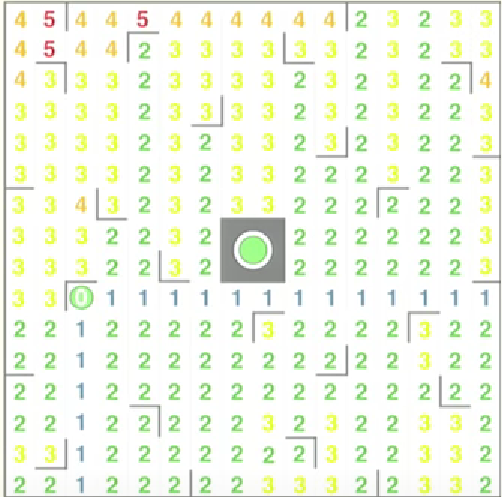
\includegraphics[width=0.5\textwidth]{init.png}  
  \caption{Exemple de grille heuristique par Randy Coulman} 
  \label{fig:Diagram}  
\end{figure}\\
En pratique, une fois l'heuristique mise en place grâce à la méthode initHeur() de la classe grid, il suffit d'appliquer l'algorithme à notre problème.
\begin{algorithm}[H]
\caption{A*}
\label{alg:dfs-reach}
\begin{algorithmic}[3]
  \STATE Entrée: noeud racine  $N$
  \STATE Créer liste $Opened$, Créer Liste $Closed$
  \STATE $Opened$.append$(N)$
  \WHILE{$Opened$ n'est pas vide}
    \STATE Enlever le noeud dont f(noeud) est minimal
    \STATE Ajouter $Closed$.append(noeud)
    \IF {noeud appartient aux noeuds finaux}
    		\RETURN Succès
    \ELSE
    		\FOR{tous les fils du noeud, noté $y$}
    			\IF{$y$ n'appartient pas à Closed union Open ou g($y$)$>$ g(noeud)+(noeud,y)}
    				\STATE g($y$) = g(noeud) + c(noeud,y)
    				\STATE f($y$) = g($y$) + h($y$)
    				\STATE pere($y$) = noeud
    				\STATE $Opened$.append$(y)$
    			\ENDIF
    		\ENDFOR
    	\ENDIF
  \ENDWHILE
  \STATE Si le but a été trouvé retourner Succès sinon retourner Echec
\end{algorithmic}
\end{algorithm}
Après des tests nous n'avons pas eu des résultats très positifs puisque le taux de réussite était presque nul. Nous avons donc implémenté une "quête secondaire". Plus précisément, avant de déplacer le robot devant aller sur la cible on place bien les autres robots. Ainsi le robot principal utilise le A* pour atteindre la cible.\\\\
Malheureusement, cet algorithme devant donner des meilleurs résultats que le BFS n'est pas abouti. Le code est disponible mais il n'est pas utilisé dans notre implémentation.
\subsubsection{Améliorations : A*}
Malgré nos difficultés pour la mise en place de cet algorithme, nous avons des pistes pour l'améliorer grandement !\\\\
On pourrait associer un poids à un état. C'est-à-dire grâce à la grille décrite dans la figure 12, on créé une méthode qui somme les poids de chaque robot. Ainsi quand on va tirer le noeud avec le poids minimal dans la liste \textit{Opened}, on choisira l'état avec le poids de plus faible.\\\\
C'est-à-dire que tous les robots se rapprocheront de la cible. Comme ça on évite l'implémentation des quêtes secondaires. On poserait évidemment une condition sur le déplacement des robots non principaux pour qu'ils ne prennent pas place sur les cases de poids strictement inférieur à deux.   
\section{Améliorations possibles du jeu}
Notre jeu est jouable dans les trois niveaux de difficulté. On peut, à la fin de chaque manche visualiser les coups qui ont été produit par l'IA.\\\\
On pourrait augmenter le nombre de manche contre l'IA durant une partie. On pourrait également générer aléatoirement de nouvelles grilles pour permettre aux joueurs de se challenger davantage et tester nos algorithmes sur ces nouvelles grilles. 
\end{document}
